\section{Clustering: warm-up}
To warm-up, we consider the classical problem of clustering artificial nodes randomly distributed
in $\mathbb{R}^{2}$ according to some geometry. More precisely, we use the package \textsf{clusterSim}
to generate 100 nodes per cluster distributed according to structures colloquially known as \textit{two-moons},
\textit{two-circles}, \textit{three-circles}, and \textit{worms}.

Figure~\ref{fig:clusters} depicts the results of learning the clusters structures using the
algorithm \textit{Spectral Graph Learning}, hereafter denoted as (\textsf{SGL}). As we can note,
\textsf{SGL} is able to perfectly distinguish the cluster membership of all the nodes for all datasets.
Additionally, Figure~\ref{fig:worms_trend} depicts the convergence trend of the terms in the objective
function for the \textit{worms} dataset.

On what concers hyperparameter selection, we use $K = 3$ for the \textit{three-circles}
dataset, otherwise we use $K = 2$. We fix $\beta = 0.25$ and $\alpha = 0$ for all the datasets.

\begin{figure}[!htb]
    \centering
    \begin{subfigure}[b]{0.23\textwidth}
      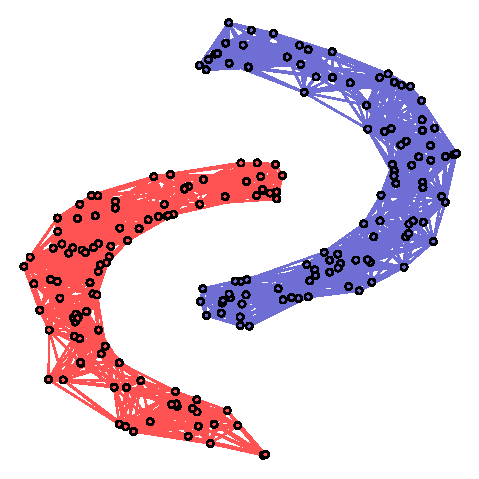
\includegraphics[width=\textwidth]{clusters/latex/figures/twomoon.eps}
      \caption{\textit{two-moons}.}
    \end{subfigure}
    ~
    \begin{subfigure}[b]{0.23\textwidth}
      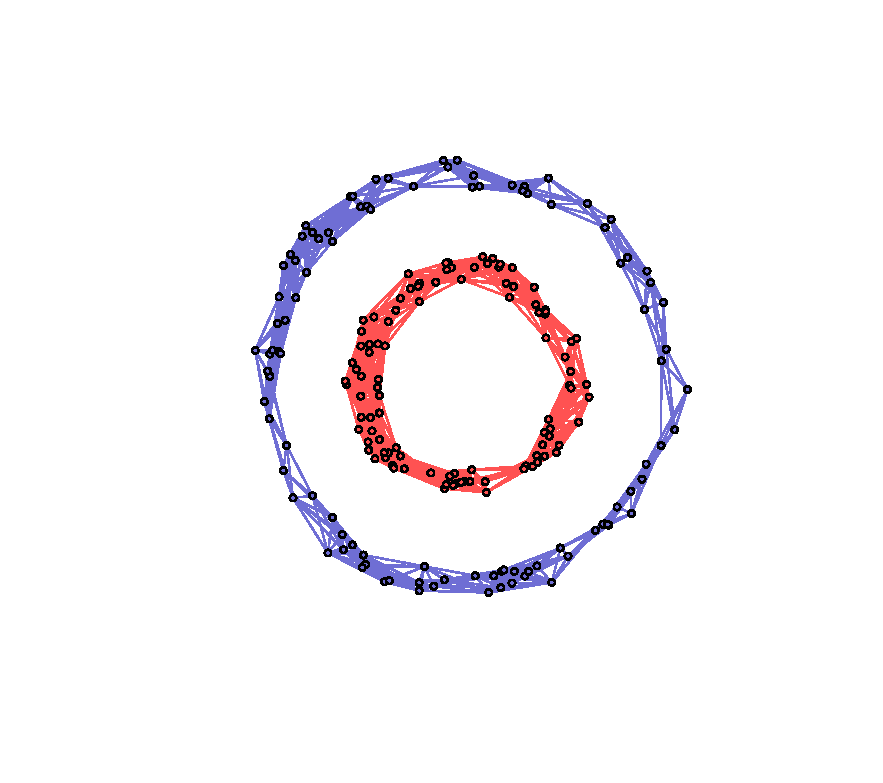
\includegraphics[width=\textwidth]{clusters/latex/figures/circles2.eps}
      \caption{\textit{two circles}.}
    \end{subfigure}
    ~
    \begin{subfigure}[b]{0.23\textwidth}
      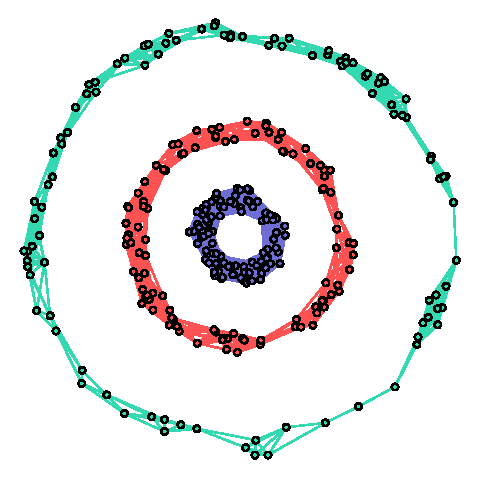
\includegraphics[width=\textwidth]{clusters/latex/figures/circles3.eps}
      \caption{\textit{three circles}.}
    \end{subfigure}
    \begin{subfigure}[b]{0.23\textwidth}
      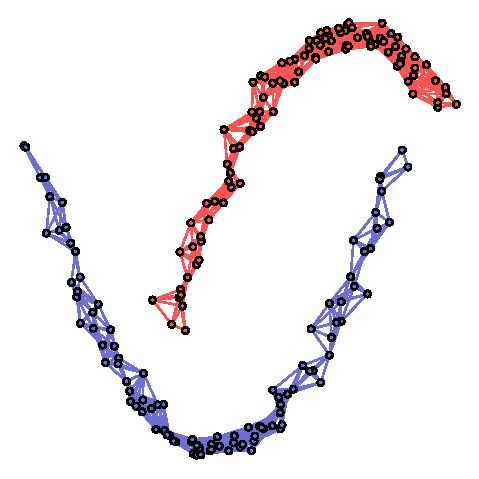
\includegraphics[width=\textwidth]{clusters/latex/figures/worms.eps}
      \caption{\textit{worms}.}
    \end{subfigure}
    \caption{Clustering results learned by the \textsf{SGL} algorithm for synthethic datasets.}
    \label{fig:clusters}
\end{figure}

\begin{figure}[!htb]
  \centering
  \includegraphics[width=.5\textwidth]{clusters/latex/figures/worms_trend.eps}
  \caption{Convergence trend of the \textsf{SGL} algorithm for the \textit{worms} dataset.}
  \label{fig:worms_trend}
\end{figure}
